\documentclass[nobib]{tufte-handout}

\usepackage{lipsum}
\usepackage{xcolor}
\usepackage{graphicx}
\usepackage{todonotes}

\newcommand{\placeholdertext}[1]{
	\noindent{\color{red}{#1}}
}

\title{Literature Review of Leading Research in Compiler Optimizations}
\author{Timothy Van Slyke}

\begin{document}
\maketitle
\section*{Abstract}
\todo{TODO: Many sections are currently just \textsf{lorem ipsum}'d and have yet to be written.  All other sections mainly consist of talking points.}
\begin{abstract}
\lipsum[1]
\end{abstract}


%%% Introduction %%%
\section{Introduction}
\todo{TODO: Collapse some of the subsections directly into the introduction and just let the discussion flow on its own.}
\lipsum[1]

\subsection{Rationale/Question/Problem}
\placeholdertext{Mobile platform power saving\ldots Modern advice is to ``get it done quickly so the device can go back to sleep''.} \newline
\placeholdertext{Desktop computing bottlenecked by memory latency} \newline
\begin{itemize}
\item There exist well-known cache-friendly access patterns but they don't always correspond with maintainable/readable code.
\end{itemize} 
\placeholdertext{Desktop computing bottlenecked by memory latency} \newline
\placeholdertext{Most if not all desktop-related rationale applies to servers.} \newline
\placeholdertext{Additionally, server farms face power consumption problems similar to those that faced by mobile platforms (but for different reasons).}

Primary question:  What new research is being done to improve software speed and efficiency at the compiler level?

%% Background %%
\subsection{Background}
Modern compilers have 

Many of the optimizations made by modern comilers for static languages like C, C++, and Java are speculative rely an conservative deductions and assumptions that said compilers can infer about the code that they analyze.  


\placeholdertext{C programmers' expectations about code generation} \ldots

\placeholdertext{JIT compilation} \ldots
\begin{itemize}
\item Popular for VM runtimes.
\item Difficult for native code.
\end{itemize}


\placeholdertext{Cache latency is one of the largest factors in program speed} \ldots



%% Methods %%
\subsection{Methods}
We've analyze publications from \placeholdertext{LIST OF CONFERENCES} \ldots


%%% Modern Compiler Optimizations %%%
\section{Modern Compiler Optimizations}
Many of the optimizations made by modern comilers for static languages like C, C++, and Java are speculative and rely an conservative deductions and assumptions that said compilers can infer about the code that they analyze.  

%% Cache-Oriented Optimizations and Memory-Bound Code %%
\subsection{Cache-Oriented Optimizations and Memory-Bound Code}
Often the most important factor that determines the speed of software on modern computer systems is the extent to which the software is able to exploit the benefits CPU cache.\footnote{This factor is relevant on both desktop and mobile platforms.  Exceptions to this rule are microcontrollers and other very small systems.}  Much work is being done to speculatively optimize code for optimal memory access patterns and to reduce CPU stall time by rerdering and eliminating memory-bound operations.

\placeholdertext{Languages with reference semantics (Java, C\#, Python) suffer poor cache performance because of their implicit object model.} \ldots \newline
\begin{itemize}
	\item Every object is dynamically allocated. 
	\item Scattered data -- no control over allocation patterns or memory layout.
\end{itemize}

\todo{TODO: Move this discussion and associated visuals to introduction/background?} Optimizing comilers for these languages suffer from few opportunities for alias analysis and must fight an uphill battle when it comes to optimizing for cache-friendly access pattens.


% Java Object Model
\begin{figure}
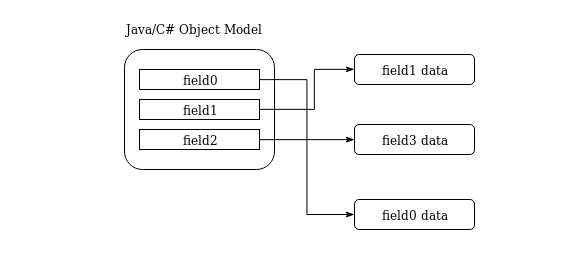
\includegraphics[width=\linewidth]{images/JavaObjectModel.png}
\caption{Visualization of the object model for languages with reference semantics.  Object fields are stored sparsely and object references are aliased liberally.  This leads to cache-unfriendly memory access patterns and poor conditions for alias analysis.}
\label{fig:JavaObjectModel}
\end{figure}

% C++ Object Model
\begin{figure}
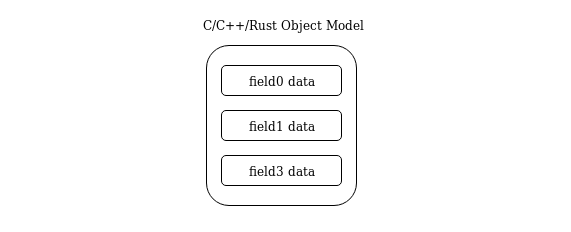
\includegraphics[width=\linewidth]{images/CppObjectModel.png}
\caption{Visualization of the object model for languages with value semantics.  Object fields are stored in a dense fashion and can only be aliased with explicit action in the code.  This leads to more cache-friendly memory access patterns and allows for reasonable alias analysis.}
\label{fig:CppObjectModel}
\end{figure}

% Python Object Model
\begin{figure}
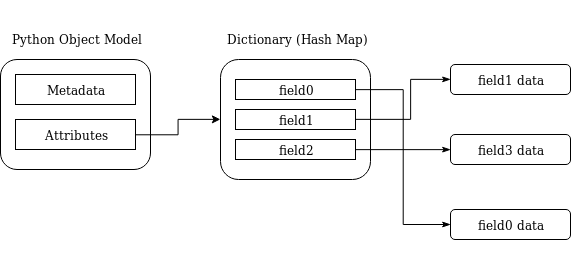
\includegraphics[width=\linewidth]{images/PythonObjectModel.png}
\caption{As a special case, the Python object model is, with only a few exceptions, implemented with a hash map; accessing object fields implies at least two layers of indirection.  This allows for highly dynamic code, but leads to extremely poor memory access patterns and makes compile-time alias analysis infeasable.} 
\label{fig:PythonObjectModel}
\end{figure}


\placeholdertext{Software Prefetching (via code generation)} \ldots \newline

\placeholdertext{Loop fusion and reordering} \ldots \newline


\subsection{Runtime Solutions}
\placeholdertext{JIT compilation} \ldots \newline

\placeholdertext{Non-JIT runtime code modification} \ldots \newline

\placeholdertext{Non-trivial code generation (compile-time)} \ldots \newline
\begin{itemize}
	\item Many source have a theme of generating runtime checks for information that cannot be known at compiler time.	
	\begin{itemize}
		\item i.e. optimization decisions made at runtime after the necessary information is made available.
	\end{itemize}
\end{itemize}
\subsection{Optimizing Parallel Code}
\placeholdertext{Automatic parallelization of code} \ldots \newline
\placeholdertext{Optimization of synchronization schemes} \ldots \newline

\subsection{Misc. or Yet-To-Be-Named Section}
\placeholdertext{Alias analysis} \ldots \newline
\placeholdertext{} \ldots \newline

\section{Results}
\lipsum[1]

\section{Conclusions}
\lipsum[1]



\newpage
\nocite{*}
\bibliographystyle{IEEEannot}
\bibliography{annot}




\end{document}

